% !TEX root = ../../prj4projektdokumentation.tex

\section{Kontrolmodul}
Kontrolmodulet består primært af to processer; En kommunikationsdel der kan håndtere at modtage data gennem en TCP forbindelse og konvertere disse data til noget der kan bruges i resten af programmet, herunder også HMI delen. En styringsdel der kan bruge disse data i styringen af trinskifteren.


\subsection{TCP kommunikation}
Kontrolmodulet er lavet som en client i forhold til kommunikationsmodulet, der er server. Den sender altså en forespørgelse på at modtage data til kommunikationsmodulet, hvorefter den modtager ny data fra den forespurgte enhed. Mere om selve protokollen kan findes i afsnit \ref{TCPprotokol} TCP protokol. Det er kontrolmodulet der oprette TCP forbindelse og står for at nedlægge den igen.

TCP komunikationen er opdelt i 4 FC'er; OpretForbindelse, SendData, ModtagData og AfslutForbindelse. Simatic TIA portal har nogle indbyggede blokke, man bruger når til Ethernetkommunikation.

OpretForbindelse består af funktionsblokken TCON, som er vist på figur \ref{fig:TCON}. Når der på REQ ses en rising edge, vil den forsøge at oprette forbindelse til en bestemt IP adresse og opretholde den, også selvom REQ bliver sat 0 igen. Forbindelse bliver vedligeholdt automatisk asynkront, så programmet kan udføre andet samtidigt. Hvis forbindelsen bliver brudt, skal REQ have en rising edge før TCON vil forsøge at oprette forbindelse igen. Datablokken Ethernet er oprettet med henblik på at indeholde globale statics anvendt i forbindelse med TCP kommunikationen, da FC'er ikke har nogen hukommelse fra scan til scan.

ID er identifikationen på forbindelsen internt i PLC'en, som de resterende blokke bruger til at identificere hvilken forbindelse er tilknyttet, hvis der skulle være flere. Her er ID sat til 1, da der kun er en forbindelse til kommunikationsmodulet.

CONNECT parameteren er en pointer til data området der indeholder forbindelsesinformation. Blokken muliggør at få informationer om forbindelsen tilstand gennem DONE, BUSY, ERROR og STATUS. Disse outputs ligger i den tilhørende DB TCON\_DB og kan kaldes gennem den. I dette projekt er der dog ikke udviklet nogen form for fejlhåndtering og disse outputs anvendes ikke. Der henvises til !!!!SYSTEM MANUAL REFERNCE!!!! for mere dybdegående forklaring af disse.

\begin{figure}[H] % (alternativt [H])
	\centering
	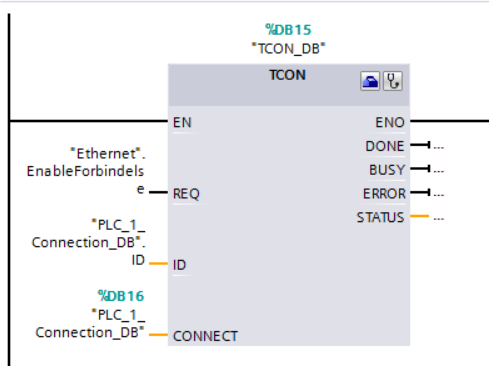
\includegraphics[width=0.5\textwidth]{Figure/TCON}
	\caption{TCON brugt i funktionen OpretForbindelse}
	\label{fig:TCON}
\end{figure}

Selve konfigureringen af hvilke enheder(IP adresser) kommunikationen skal foregå imellem sættes under properties for TCON. På figur \ref{fig:Konfiguration} kan det kan ses at på lokalsiden er PLC'en sat op til at have IP adressen 192.168.0.120, anvende TCP over subnet PN/IE\_1, som er default 255.255.255.0, samt være aktiv i forhold til at oprette forbindelsen. Feltet Connection data, fortæller hvilken Datablok der indeholder data omkring forbindelse, herunder bla. ID og CONNECT.

På partnersiden er Arduinoen ikke et Siemens modul og derfor unspecified. Her er valgt at kommunikationsmodulet har IP adressen 192.168.0.129 og bruger port 27015 til kommunikationen. Denne port er valgt af hensyn til Arduinoens præferencer i forhold til mulige porte.

\begin{figure}[H] % (alternativt [H])
	\centering
	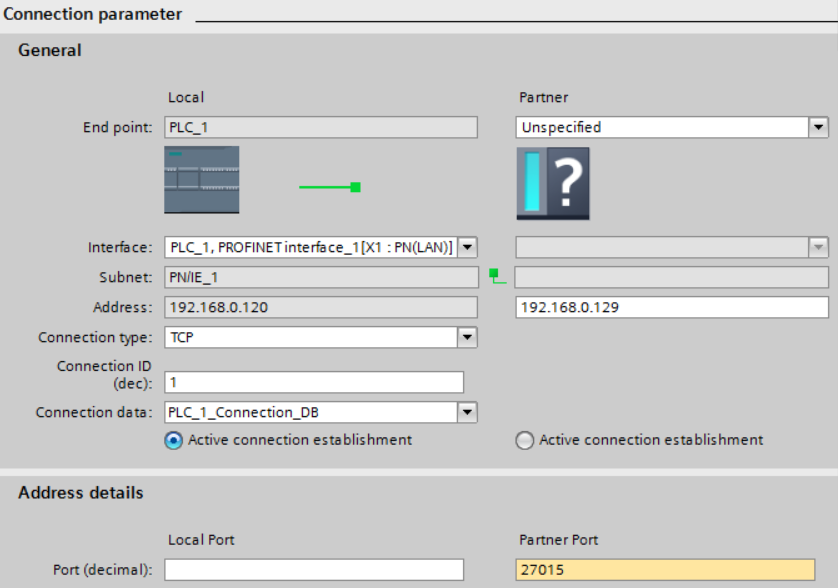
\includegraphics[width=0.7\textwidth]{Figure/KonfigurationAfTCPforbindelse}
	\caption{Konfiguration af TCP forbindelse}
	\label{fig:Konfiguration}
\end{figure}

Funktionen AfslutForbindelse står for at nedlægge forbindelse. Da der kun kommunikeres med en enhed, anvender programmet dog aldrig denne mulighed. Alligevel er funktionen lavet for at det er nemt at videreudvikle, med henblik på at tilføje flere TCP forbindelser. 

Funktionsblokken TDISCON anvendes til denne opgave. Når blokkens REQ ser en rsing edge nedlægges forbindelsen og det vil kræve en rising edge på TCON's REQ for at genetablere forbindelsen. Blokken skal også bruge et ID på forbindelse, ID'et er sat i konfigurationen af TCON. Her kan man også få informationer omkring blokken gennem DONE, BUSY, ERROR og STATUS. Igen anvendes disse ikke, da der ikke er lagt vægt på fejlhåndtering i dette projekt. De kan kaldes gennem datablokken TDISCON\_DB. Der henvises til !!!!SYSTEM MANUAL REFERNCE!!!! for mere dybdegående forklaring af disse.

\begin{figure}[H] % (alternativt [H])
	\centering
	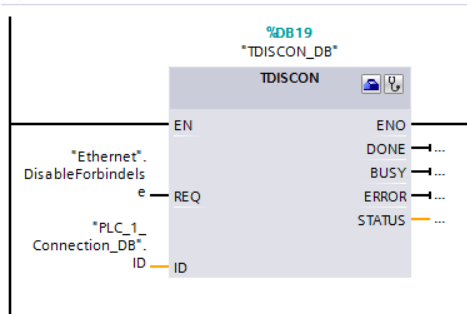
\includegraphics[width=0.5\textwidth]{Figure/TDISCON}
	\caption{TDISCON brugt i funktionen AfslutForbindelse}
	\label{fig:TDISCON}
\end{figure}

Når forbindelsen er oprettet bruges funktionerne SendData og ModtagData til  kommunikering af data. SendData anvender funktioneblokken TSEND til at afsende data placeret i den globale static SendData. Når REQ modtager en rising edge afsendes dataet. Mens ID igen specificerer hvilken forbindelse, der skal sendes over.

Ligesom TCON og TDISCON anvendes DONE, BUSY, ERROR og STATUS ikke.

\begin{figure}[H] % (alternativt [H])
	\centering
	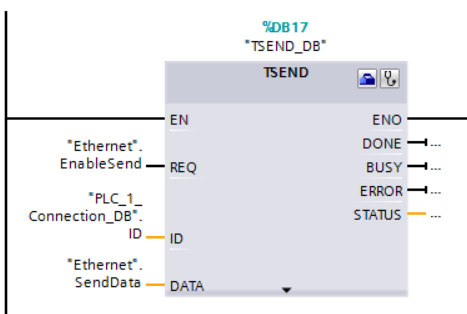
\includegraphics[width=0.5\textwidth]{Figure/TSEND}
	\caption{TSEND brugt i funktionen SendData}
	\label{fig:TSEND}
\end{figure}

Til at styre hvor ofte der forespørges ny data og hvilken enhed der forespørges data fra, er designet et netværk, hvor en global static boolean Firsttime sættes true før send processen sættes igang. Firsttime bliver sat true når data er modtaget og gemt. Den er defualt true ellers vil det blokere programmet i kraft af at PLC'en ikke modtager data før den har sendt en kommando på ny data.

Når Firsttime er sat igangsættes netværket vist på figur \ref{fig:ValgAfEnhedSend}. Her resettes den static der styrer REQ på TSEND og en on delay timer startes. Timere anvendes i programmet for kunne styre hvor ofte der hentes ny data. For systemet der udvikles er det ikke nødvendigt at dette går hurtigt. Så det blev besluttet at data fra både den centrale og den decentrale måleenheder skulle opdateres hver 2 sekunder. Derfor er der valgt en timer på 500ms i både SendData og ModtagData funktionen.

Når First

\begin{figure}[H] % (alternativt [H])
	\centering
	\includegraphics[width=1\textwidth]{Figure/valgAfEnhedSend}
	\caption{Netværket der styrer hvilken enhed der forespørges data fra}
	\label{fig:ValgAfEnhedSend}
\end{figure}

\begin{figure}[H] % (alternativt [H])
	\centering
	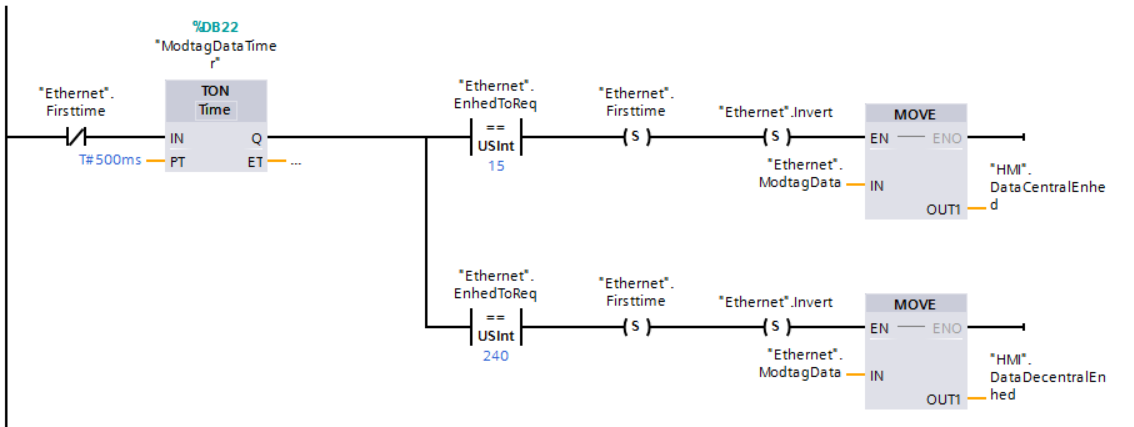
\includegraphics[width=1\textwidth]{Figure/GemModtagetData}
	\caption{Netværket der gemmer modtagede data}
	\label{fig:TSEND}
\end{figure}

\begin{figure}[H] % (alternativt [H])
	\centering
	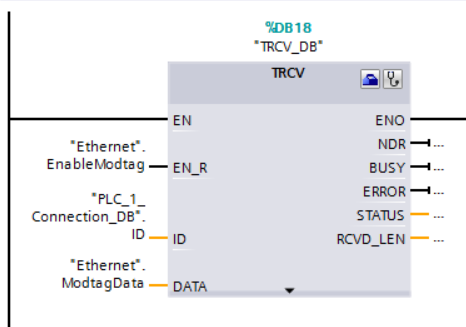
\includegraphics[width=0.5\textwidth]{Figure/TRCV}
	\caption{TRCV brugt i funktionen ModtagData}
	\label{fig:TRCV}
\end{figure}


\subsection{Styring af trinskifter}